\chapter{Bug fixing and new features}\label{chap:chap3}

\epigraph{``If debugging is the process of removing software bugs, then programming must be the process of putting them in.''}{\textit{Edsger W. Dijkstra}}

\subsection*{Getting the project to a working state}

\paragraph*{The flag setting bug}

In LEGv8, CMP and CMPI are pseudoinstructions, meaning that under the hood they actually make use of the SUBS and SUBIS instructions respectively to set the compare flags. The fact that the former instructions failed, pointed at a problem in the latter ones, which was proven to be correct. The simulator first implements the function responsible for setting the flags of the addition operations and when setting the flags for the subtraction operations it simply calls the same function with the same arguments.
\begin{lstlisting}[caption={The adddition flag-setting code}]
	private void ADDSetFlags(long result, long op1, long op2) {
		setNflag(result < 0);
		setZflag(result == 0);
		setCflag(result, op1, op2);
		setVflag(result, op1, op2);
	}
\end{lstlisting}
\begin{lstlisting}[caption={The buggy subtraction flag-setting code}]
	private void SUBSetFlags(long result, long op1, long op2) {
		ADDSetFlags(result, op1, op2);
	}
\end{lstlisting}
As we can see, this presents a problem since subtraction and addition set their flags in a different way. The fix was simply to call the same function but with the 2-complement of the second operand.
\begin{lstlisting}[caption={The fixed subtraction flag-setting code}]
	private void SUBSetFlags(long result, long op1, long op2) {
		ADDSetFlags(result, op1, (~op2)+1);
	}
\end{lstlisting}

\paragraph*{The branch return bug}

For this bug, inspecting the LR register showed that the BL instruction was not writing the register with the address of the current instruction, but with the subroutine's one instead. This created an infinite loop since, when the subroutine returned to the LR, the program would jump back to the beginning of the subroutine all over again.
\begin{lstlisting}[caption={The buggy address writing}]
	private void BL(int branchIndex) {
		instructionIndex = branchIndex;
		XRegisterFile[LR].writeDoubleWord(instructionIndex * INSTRUCTION_SIZE + Memory.TEXT_SEGMENT_OFFSET);
		...
	}
\end{lstlisting}
As we can see, the instructionIndex is updated too soon and thus the LR register gets written with the address of the branch.
\begin{lstlisting}[caption={The fixed address writing}]
	private void BL(int branchIndex) {
		XRegisterFile[LR].writeDoubleWord(instructionIndex * INSTRUCTION_SIZE + Memory.TEXT_SEGMENT_OFFSET);
		instructionIndex = branchIndex;
		...
	}
\end{lstlisting}

\paragraph*{The datapath visualization bug}
An issue that was raised on GitHub \footnote{\url{https://github.com/arm-university/Graphical-Micro-Architecture-Simulator/issues/8}} complained about erroneous values of the MemWrite and MemRead signals from the control unit. This was a problem in the configuration.
\begin{lstlisting}[caption={Buggy SingleCycleVis.java}]
	...
	ctx.fillText(ControlUnitConfiguration.toString(c.memRead), DATA_MEM_COORDS[0]+DATA_MEM_DIMENSIONS[0]/2-t.getWidth()-1, DATA_MEM_COORDS[1]-3);
	ctx.fillText(ControlUnitConfiguration.toString(c.memToReg), MUX_READ_DATA_MEM_COORDS[0]+MUX_READ_DATA_MEM_DIMENSIONS[0]/2-t.getWidth()-1, MUX_READ_DATA_MEM_COORDS[1]-3);
	ctx.fillText(ControlUnitConfiguration.toString(c.memRead), DATA_MEM_COORDS[0]+DATA_MEM_DIMENSIONS[0]/2-t.getWidth()-1, DATA_MEM_COORDS[1]+DATA_MEM_DIMENSIONS[1]+10);
	...
\end{lstlisting}
\begin{lstlisting}[caption={Fixed SingleCycleVis.java}]
	...
	ctx.fillText(ControlUnitConfiguration.toString(c.memWrite), DATA_MEM_COORDS[0]+DATA_MEM_DIMENSIONS[0]/2-t.getWidth()-1, DATA_MEM_COORDS[1]-3);
	ctx.fillText(ControlUnitConfiguration.toString(c.memToReg), MUX_READ_DATA_MEM_COORDS[0]+MUX_READ_DATA_MEM_DIMENSIONS[0]/2-t.getWidth()-1, MUX_READ_DATA_MEM_COORDS[1]-3);
	ctx.fillText(ControlUnitConfiguration.toString(c.memRead), DATA_MEM_COORDS[0]+DATA_MEM_DIMENSIONS[0]/2-t.getWidth()-1, DATA_MEM_COORDS[1]+DATA_MEM_DIMENSIONS[1]+10);
	...
\end{lstlisting}
\begin{lstlisting}[caption={BuggyControlUnitConfiguration.java}]
	...
	RM_LOAD(null, false, false, false, false, true, true, false, true, 0, true),
	...
\end{lstlisting}
\begin{lstlisting}[caption={Fixed ControlUnitConfiguration.java}]
	...
	RM_LOAD(null, false, false, false, true, true, false, false, true, 0, true),
	...
\end{lstlisting}

\subsection*{Adding new features}

\paragraph{Refactoring the memory}

The \verb|ByteBuffer.java| and \verb|Memory.java| classes have mostly been left untouched, although their methods and variables presented some Java-centric names and have thus been replaced with more apt LEGv8 names such as \verb|getDoubleWord| instead of \verb|getLong|. The base address of the stack, defined in the textbook as \verb|0x7ffffffffc|,  was not quadword-aligned, leading to a design contradiction. I chose to change it to the  compatible address \verb|0x8000000000|.

\paragraph{Completing the integer arithmetic}

The integer-related instructions missing from the simulator were: \verb|MUL|, \verb|SMULH|, \verb|UMULH|, \verb|SDIV|, and \verb|UDIV|. In order to implement these new instructions a few changes to the code had to be made. First of all they had been added to \verb|Mnemonic.java|.
\begin{lstlisting}[caption={Added mnemonics}]
	...
	MUL("MUL", "mul", TokenType.XMNEMONIC_RRR, "10011011000", "0010"),
	SMULH("SMULH", "smulh", TokenType.XMNEMONIC_RRR, "10011011010", "0010"),
	UMULH("UMULH", "umulh", TokenType.XMNEMONIC_RRR, "10011011110", "0010"),
	SDIV("SDIV", "sdiv", TokenType.XMNEMONIC_RRR, "10011010110", "0010")
	UDIV("UDIV", "udiv", TokenType.XMNEMONIC_RRR, "10011010110", "0010"),
	...
\end{lstlisting}
Then to Decoder.java
\begin{lstlisting}[caption={Added instructions to the decoder}]
	...
	case MUL :
	return new Instruction(mnemonic, decodeRRRArgs(args), lineNumber, ControlUnitConfiguration.RRR);
	case UMULH :
	return new Instruction(mnemonic, decodeRRRArgs(args), lineNumber, ControlUnitConfiguration.RRR);
	case SMULH :
	return new Instruction(mnemonic, decodeRRRArgs(args), lineNumber, ControlUnitConfiguration.RRR);
	case UDIV :
	return new Instruction(mnemonic, decodeRRRArgs(args), lineNumber, ControlUnitConfiguration.RRR);
	case SDIV :
	return new Instruction(mnemonic, decodeRRRArgs(args), lineNumber, ControlUnitConfiguration.RRR);
	...
\end{lstlisting}
Then they had to be added to \verb|TokenType.java| to use with the parser
\begin{lstlisting}[caption={Addition to the parser}]
	...
		MNEMONIC_RRR("ADDS?[ \t]+|SUBS?[ \t]+|ANDS?[ \t]+|MUL[ \t]+|SMULH[ \t]+|UMULH[ \t]+|SDIV[ \t]+|UDIV[ \t]+|ORR[ \t]+|EOR[ \t]+|adds?[ \t]+|subs?[ \t]+|ands?[ \t]+|mul[ \t]+|smulh[ \t]+|umulh[ \t]+|sdiv[ \t]+|udiv[ \t]+|orr[ \t]+|eor[ \t]+", 15, "MNEMONIC"),
	...
\end{lstlisting}
And finally they had to be implemented inside \verb|CPU.java| to execute the operations
\begin{lstlisting}[caption={}]
	...
	private void MUL(int destReg, int op1Reg, int op2Reg) {											
			XRegisterFile[destReg].writeDoubleWord(XRegisterFile[op1Reg].readDoubleWord() * XRegisterFile[op2Reg].readDoubleWord());
		}
	}
	private void SDIV(int destReg, int op1Reg, int op2Reg) {
			XRegisterFile[destReg].writeDoubleWord(XRegisterFile[op1Reg].readDoubleWord() / XRegisterFile[op2Reg].readDoubleWord());
	}
	
	private void UDIV(int destReg, int op1Reg, int op2Reg) {
			BigInteger dividend = BigInteger.valueOf(XRegisterFile[op1Reg].readDoubleWord()).and(UNSIGNED_LONG_MASK);
			BigInteger divisor = BigInteger.valueOf(XRegisterFile[op2Reg].readDoubleWord()).and(UNSIGNED_LONG_MASK);
			BigInteger quotient = dividend.divide(divisor);
			XRegisterFile[destReg].writeDoubleWord(quotient.longValue());
	}
	
	private void SMULH(int destReg, int op1Reg, int op2Reg) {
			BigInteger fullResult = BigInteger.valueOf(XRegisterFile[op1Reg].readDoubleWord()).multiply(BigInteger.valueOf(XRegisterFile[op2Reg].readDoubleWord()));
			BigInteger shiftedResult = fullResult.bitLength() > 64 ? fullResult.shiftRight(64) : BigInteger.valueOf(0);
			XRegisterFile[destReg].writeDoubleWord(shiftedResult.longValue());;
			
	}
	
	private void UMULH(int destReg, int op1Reg, int op2Reg) {
			BigInteger fullResult = BigInteger.valueOf(XRegisterFile[op1Reg].readDoubleWord()).and(UNSIGNED_LONG_MASK).multiply(BigInteger.valueOf(XRegisterFile[op2Reg].readDoubleWord()).and(UNSIGNED_LONG_MASK));
			BigInteger shiftedResult = fullResult.bitLength() > 64 ? fullResult.shiftRight(64) : BigInteger.valueOf(0);
			XRegisterFile[destReg].writeDoubleWord(shiftedResult.longValue());;
	}
	...
\end{lstlisting}
Of particular interest are the \verb|UDIV|, \verb|UMULH| and \verb|SMULH| instructions as they make use of the \verb|BigInteger| class.
\begin{itemize}
\item Java does not support unsigned integers. This means that \verb|UDIV| needs to artificially represent them with 65 bit signed numbers through the use of a bit mask. This way it's able to perform the division and return a native 64 bit signed integer.
\item The \verb|*MULH| instructions perform a 128-bit multiplication between two 64-bit integers and retain the higher 64 bits. To perform such a calculation Java needs to go beyond its primitive types and make use of \verb|BigInteger|.
\end{itemize}
Of course this could have been done in more primitive ways through the use of arrays, but GWT supported the \verb|BigInteger| type and allowed to solve the problem quickly.

\subparagraph*{Finishing touches}
The last integer (pseudo)instruction to be implemented was \verb|LDA|. Its purpose is to copy the address pointed by a label into a register. Since the instruction follows the same format as \verb|CBZ| and \verb|CBNZ| (i.e. its arguments are an \verb|X| register and a label), it was added as an \verb|RL|-type instruction and by reading the address of the label from the branch table \footnote{A table populated by the CPU both statically and dynamically that associates each label to its address}. I should note that the LEGv8 documentation seems to be inconsistent in its description of this pseudo-instruction. In fact, from how it is talked about in the textbook, it seems to do what I have described above, but when looking at the LEGv8 reference guide it's described as \verb|R[Rd] = R[Rn] + DTAddress|, implying that it actually operates by taking the value of a register \verb|Rn|, adding it to the address \verb|DTAddress| specified by the label, and then writing the result into the \verb|Rd| destination address. Furthermore, this instruction is present in just a couple of LEGv8 examples and never explained in detail, so I decided to implement it following the examples in the book instead of its formal specification.

\paragraph*{Visualizing the stack}

After finishing implementing the integer arithmetic it was time to make the stack visible inside the web interface. This was done by reutilizing the same structure of \verb|RegisterPanel.java|. As it's evident from \verb|StackPanel.java|, the stack visualization includes the address of the double word stored and only shows hexadecimal values, unlike with \verb|X| registers where you can convert between hex and decimal signed representation.

\begin{figure}[H]
	\centering
	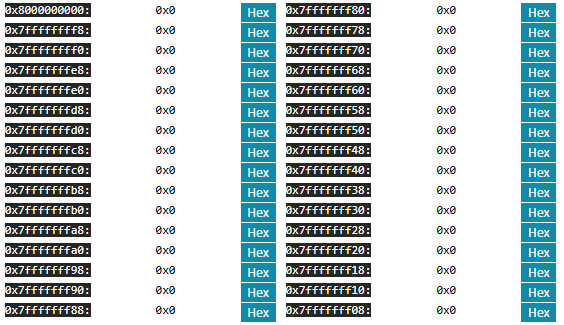
\includegraphics[width=.8\textwidth]{img/stack_vis.png}
	\caption{The newly introduced stack visualization}
\end{figure}

\paragraph*{Implementing floating point arithmetic}

Since the simulator was built with integer arithmetic in mind, all the additions made until now did not require any change to the underlying logic and structure of the code base. Introducing floating point operations on the other hand, required updating other parts of the logic that were previously left untouched.

\subparagraph*{Adding floating point registers}

The introduction of two new types of registers required the creation of a new \verb|Register.java| type. This new class includes the \emph{type} of the register, its \emph{content} (i.e. the bits stored inside) and the methods to write and read from it. I have chosen to memorize the bits inside of the registers as a \verb|long| value regardless of the register type. This is because Java offers utility methods to convert \verb|float|s into \verb|int| bits, \verb|double|s into \verb|long| bits, and vice versa, I simply applied these conversions when reading and writing to the registers. This way, the \verb|long| and \verb|int| values used throughout the simulator become just sequences of bits without an implicit interpretation. Although this choice might not be obvious when reading the code since no binary type was introduced, one of its advantages has been that the \verb|Memory.java| class has not required any changes to keep working correctly.

\subparagraph*{Adding floating point operations}

Having added the new registers to \verb|CPU.java|, it was now possible to implement all the floating point operations. Just like before, different classes had to be modified, but right now I will focus on the operations done by the CPU.

	\begin{lstlisting}[caption={FADDS}]
		...
		DRegisterFile[destReg].writeWord(Float.floatToIntBits(
		Float.intBitsToFloat(DRegisterFile[op1Reg].readWord()) +
		Float.intBitsToFloat(DRegisterFile[op2Reg].readWord())
		));
		...
	\end{lstlisting}
	\begin{lstlisting}[caption={FADDD}]
		...
		DRegisterFile[destReg].writeDoubleWord(Double.doubleToLongBits(
		Double.longBitsToDouble(DRegisterFile[op1Reg].readDoubleWord()) +
		Double.longBitsToDouble(DRegisterFile[op2Reg].readDoubleWord())
		));
		...
	\end{lstlisting}
	\begin{lstlisting}[caption={FCMPS}]
		...
		float op1f = Float.intBitsToFloat(DRegisterFile[op1Reg].readWord());
		float op2f = Float.intBitsToFloat(DRegisterFile[op2Reg].readWord());
		FCMPSetFlags(Float.compare(op1f, op2f), Float.isNaN(op1f) || Float.isNaN(op1f));
		...
	\end{lstlisting}
	\begin{lstlisting}[caption={FCMPD}]
		...
		double op1d = Double.longBitsToDouble(DRegisterFile[op1Reg].readDoubleWord());
		double op2d = Double.longBitsToDouble(DRegisterFile[op2Reg].readDoubleWord());
		FCMPSetFlags(Double.compare(op1d, op2d), Double.isNaN(op1d) || Double.isNaN(op2d));
		...
	\end{lstlisting}
	\begin{lstlisting}[caption={Function for setting floating point comparison flags}]
		private void FCMPSetFlags(int comparisonResult, boolean isNaN) {
			setNflag(comparisonResult < 0 && !isNaN);
			setZflag(comparisonResult == 0 && !isNaN);
			setCflag(comparisonResult >= 0 || isNaN);
			setVflag(isNaN);
		}
	\end{lstlisting}
	
	It's important to note that the LEGv8 specification does not say how flags should be set in case of floating point comparison. As a guideline my supervisor Prof. Carini decided to use ARM's official documentation regarding IEEE 754 \footnote{\url{https://community.arm.com/arm-community-blogs/b/architectures-and-processors-blog/posts/condition-codes-4-floating-point-comparisons-using-vfp}}. Since Java offers the same comparison utility methods and criteria for single and double precision floating point numbers, a single method needed to be written.
	
	\begin{figure}[H]
		\centering
		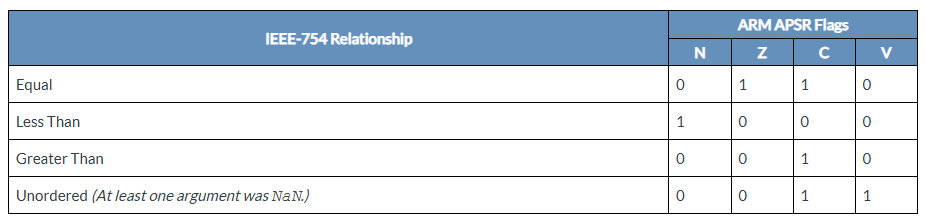
\includegraphics[width=.8\textwidth]{img/ieee754_flags.png}
		\caption{The flag setting convention for floating point comparisons.}
	\end{figure}
	
	\begin{lstlisting}[caption={FDIVS}]
		...
		DRegisterFile[destReg].writeWord(Float.floatToIntBits(
		Float.intBitsToFloat(DRegisterFile[op1Reg].readWord()) /
		Float.intBitsToFloat(DRegisterFile[op2Reg].readWord())
		));
		...
	\end{lstlisting}
	\begin{lstlisting}[caption={FDIVD}]
		...
		DRegisterFile[destReg].writeDoubleWord(Double.doubleToLongBits(
		Double.longBitsToDouble(DRegisterFile[op1Reg].readDoubleWord()) /
		Double.longBitsToDouble(DRegisterFile[op2Reg].readDoubleWord())
		));
		...
	\end{lstlisting}
	\begin{lstlisting}[caption={FMULS}]
		...
		DRegisterFile[destReg].writeWord(Float.floatToIntBits(
		Float.intBitsToFloat(DRegisterFile[op1Reg].readWord()) *
		Float.intBitsToFloat(DRegisterFile[op2Reg].readWord())
		));
		...
	\end{lstlisting}
	\begin{lstlisting}[caption={FMULD}]
		...
		DRegisterFile[destReg].writeDoubleWord(Double.doubleToLongBits(
		Double.longBitsToDouble(DRegisterFile[op1Reg].readDoubleWord()) *
		Double.longBitsToDouble(DRegisterFile[op2Reg].readDoubleWord())
		));
		...
	\end{lstlisting}
	\begin{lstlisting}[caption={FSUBS}]
		...
		DRegisterFile[destReg].writeWord(Float.floatToIntBits(
		Float.intBitsToFloat(DRegisterFile[op1Reg].readWord()) -
		Float.intBitsToFloat(DRegisterFile[op2Reg].readWord())
		));
		...
	\end{lstlisting}
	\begin{lstlisting}[caption={FSUBD}]
		...
		DRegisterFile[destReg].writeDoubleWord(Double.doubleToLongBits(
		Double.longBitsToDouble(DRegisterFile[op1Reg].readDoubleWord()) -
		Double.longBitsToDouble(DRegisterFile[op2Reg].readDoubleWord())
		));
		...
	\end{lstlisting}
	
	As we can see from the last four instructions, the floating point registers, just like their integer counterpart, write and read values from the memory in the exact same way without any change to the logic. In fact, these methods could be refactored and grouped together to reduce code duplication.
	
	\begin{lstlisting}[caption={LDURS}]
		...
		DRegisterFile[destReg].writeWord((int) memory.loadDoubleword(XRegisterFile[baseAddressReg].readDoubleWord()+offset));
		...
	\end{lstlisting}
	\begin{lstlisting}[caption={LDURD}]
		...
		DRegisterFile[destReg].writeDoubleWord(memory.loadDoubleword(XRegisterFile[baseAddressReg].readDoubleWord()+offset));
		...
	\end{lstlisting}
	
	\begin{lstlisting}[caption={STURS}]
		...
		memory.storeWord(XRegisterFile[baseAddressReg].readDoubleWord()+offset, DRegisterFile[valReg].readDoubleWord());
		...
	\end{lstlisting}
	\begin{lstlisting}[caption={STURD}]
		...
		memory.storeDoubleword(XRegisterFile[baseAddressReg].readDoubleWord()+offset, DRegisterFile[valReg].readDoubleWord());
		...
	\end{lstlisting}

\subparagraph*{Refactoring the parser}

LEGv8 does not allow instructions to operate on different types of registers. For this reason code like \verb|ADD X0, S4, D20| or \verb|FADDS X0, X1, X2| is not valid. This in turn means that the assembler (in this case, the parser) needs to be made aware that certain instructions work only with certain types of registers. 
\newline
The parser works by implementing a finite state machine through the use of enumerators. It takes each line and scans it step by step to check if its syntax is correct. The integer parser has the following diagram.

\begin{figure}[H]
	\centering
	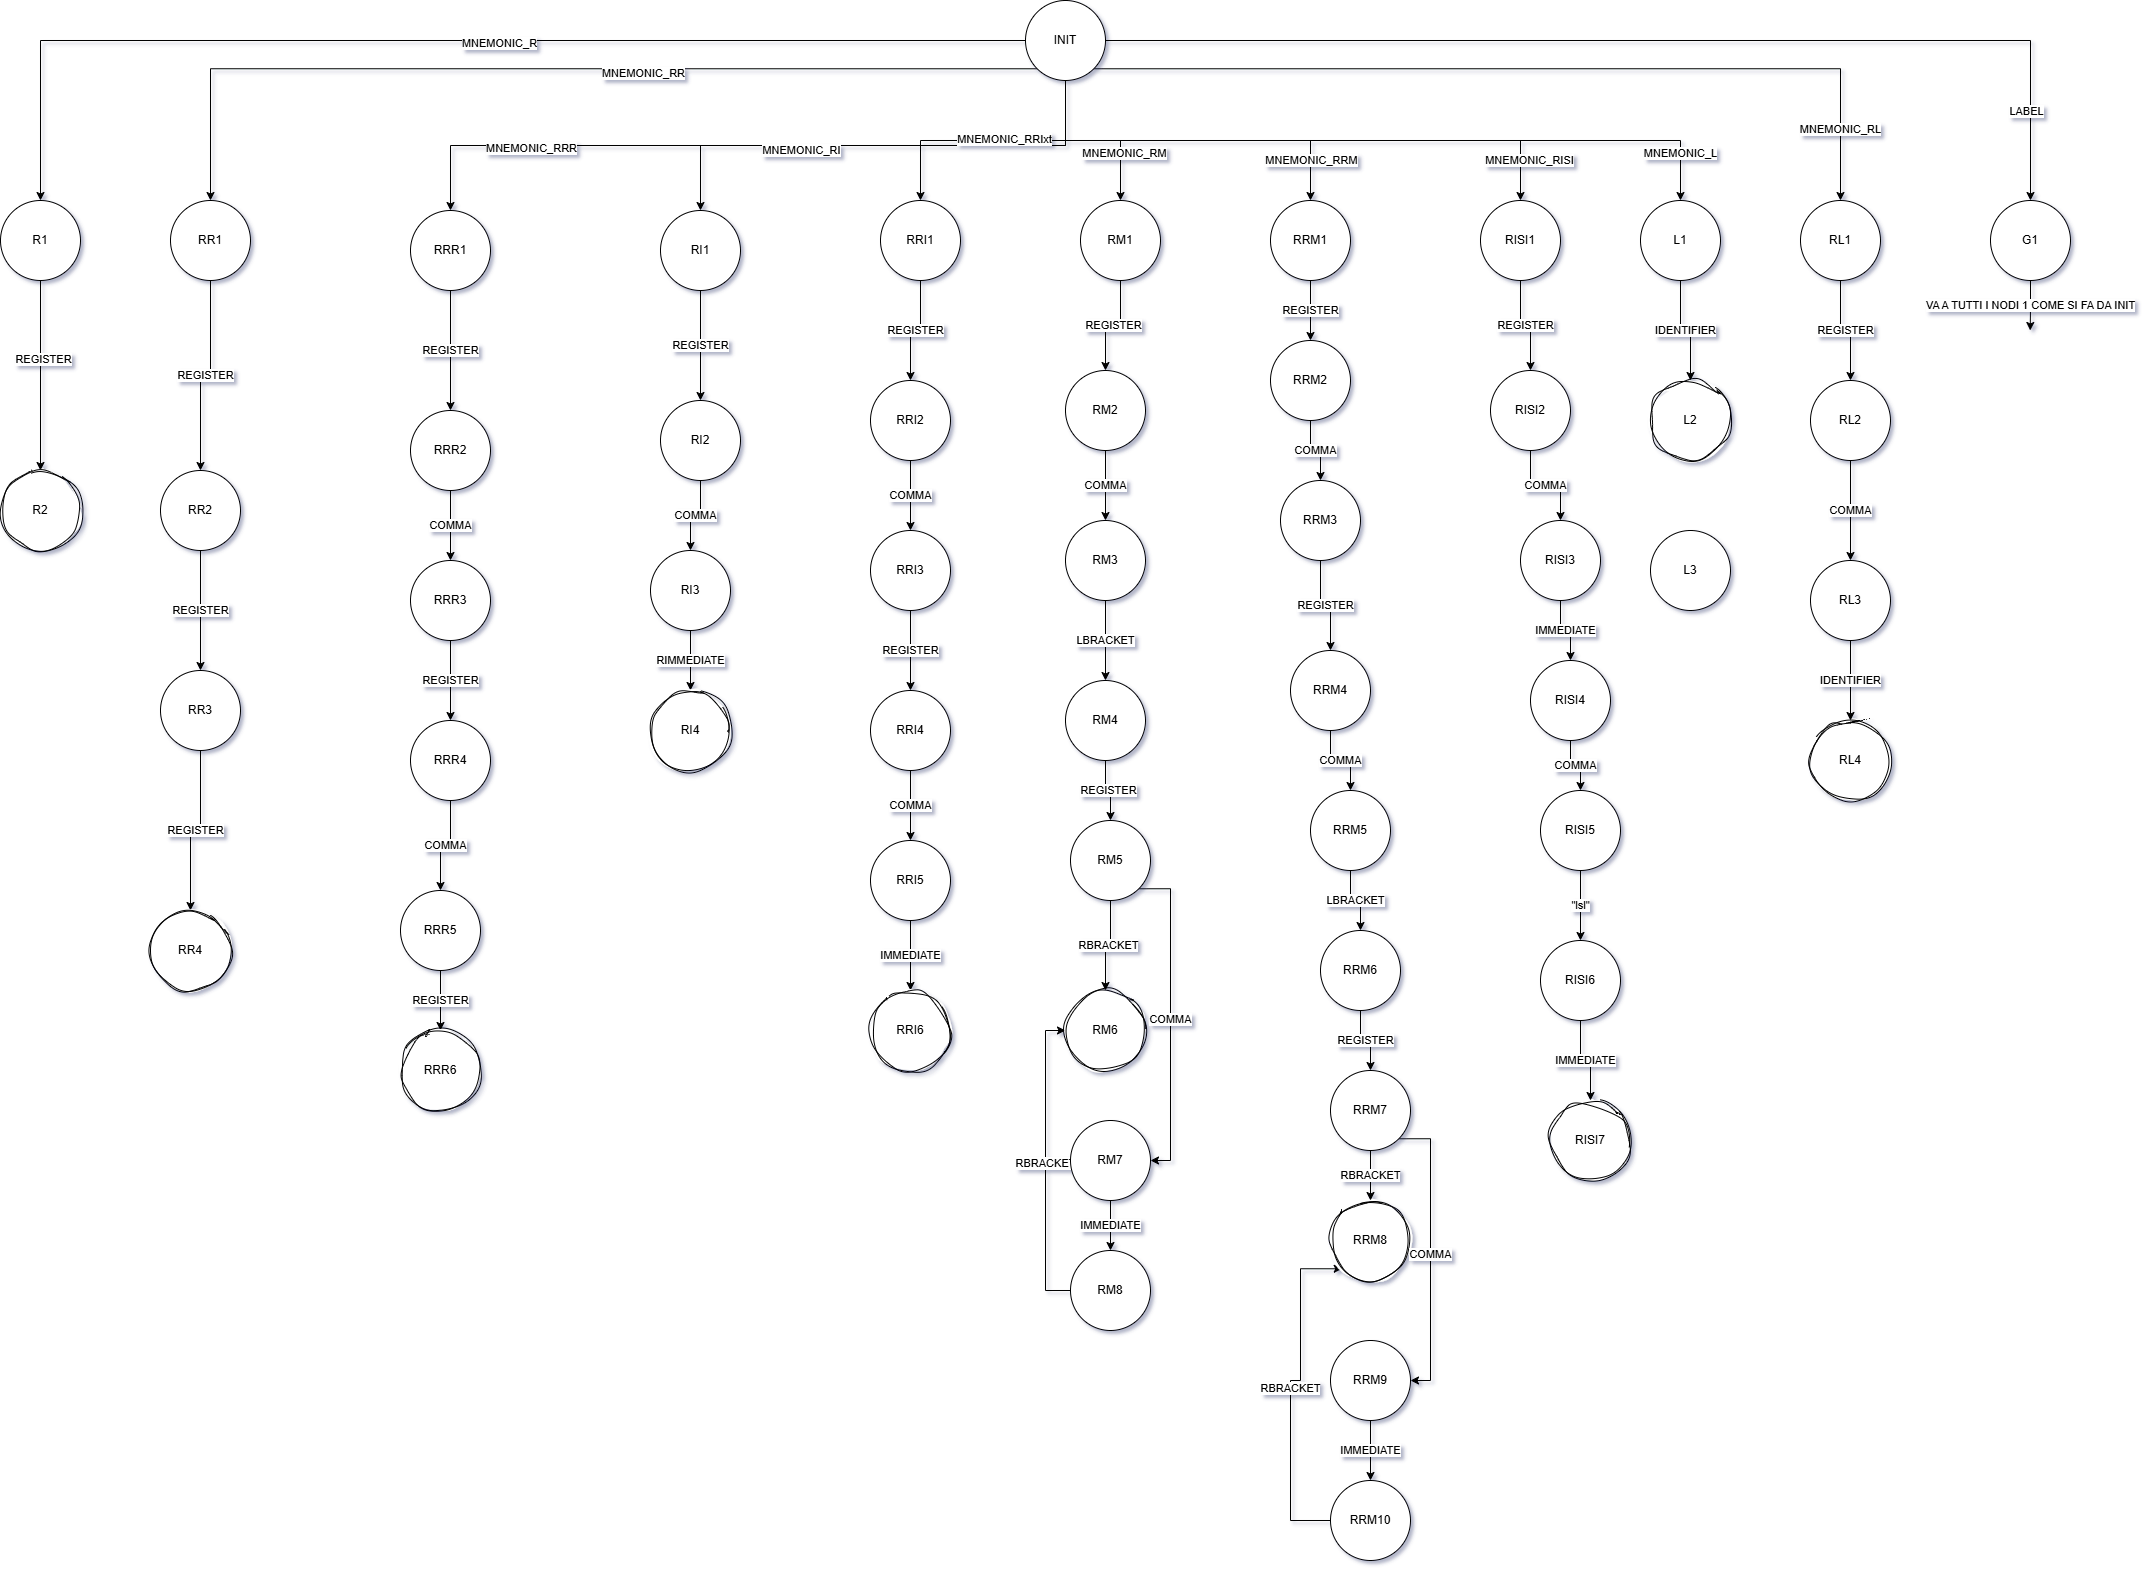
\includegraphics[width=\textwidth]{img/parser_diagram.png}
	\caption{The old integer-instructions-only parser.}
\end{figure}

The structure of the parser allows it to be extended quite easily. This was done by recategorizing all the mnemonics into \verb|X|, \verb|S|, and \verb|D| type mnemonics. For example, what once was a \verb|MNEMONIC_RRR| (i.e. an instruction that operates on 3 registers), now is split into \verb|XMNEMONIC_RRR|,  \verb|SMNEMONIC_RRR|, and  \verb|DMNEMONIC_RRR|, each of them being able to oeprate only on the compatible registers. By doing this, the parser now recognizes invalid hybrid instructions and refuses to run the program.

\subparagraph*{Visualizing the new registers}

Adding the visualization for the new registers required similar work as what was done with the displaying of the stack. A new \verb|FloatRegisterPanel.java| class was created following the same structure as the integer registers'. The only real change besides the registers' labels was to correctly display the decimal representation of the floating point number stored inside the register.

\subparagraph*{Visualizing the data path}

The only thing left was to refactor the \verb|SingleCycleVis.java| class to make it recognize the new types of mnemonics and thus provide a correct visualization for the kinds of operations they were performing.

\subparagraph*{Updating the pipelined view}

Even though the pipelined execution wasn't a subject of my work, I decided to at least change the visualization to include the new registers and stack view and to make it more organized inside the web page.

\subsection*{The final look}

\begin{figure}[H]
	\centering	
	\subfigure[New single cycle]{
		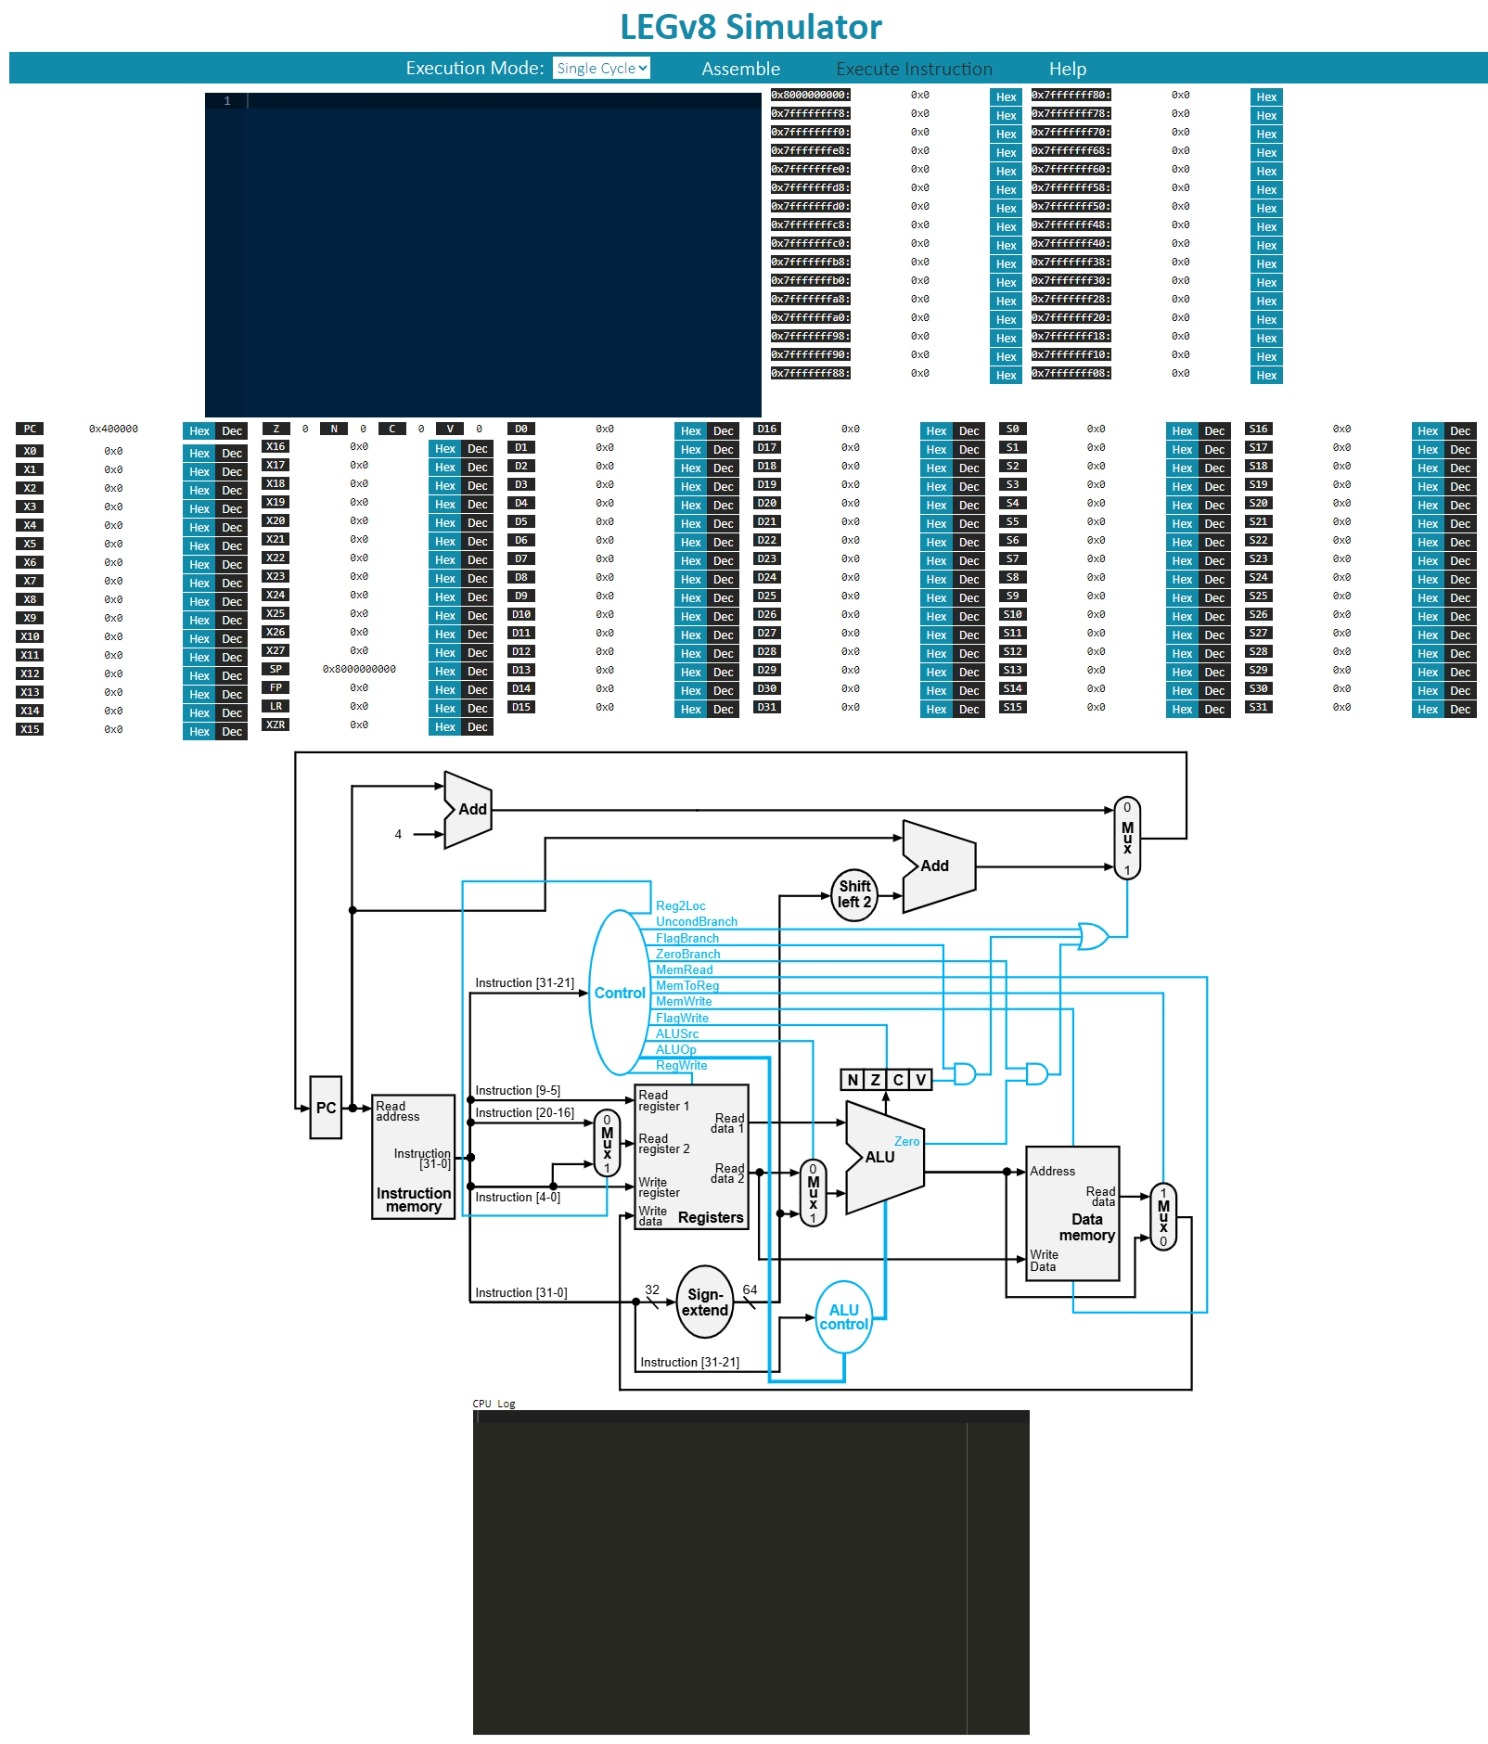
\includegraphics[width=1\textwidth]{img/new_single_cycle.jpeg}
	}
	\caption{The updated single cycle UI}
\end{figure}

\begin{figure}[H]
	\centering
	\subfigure[New pipeline]{
		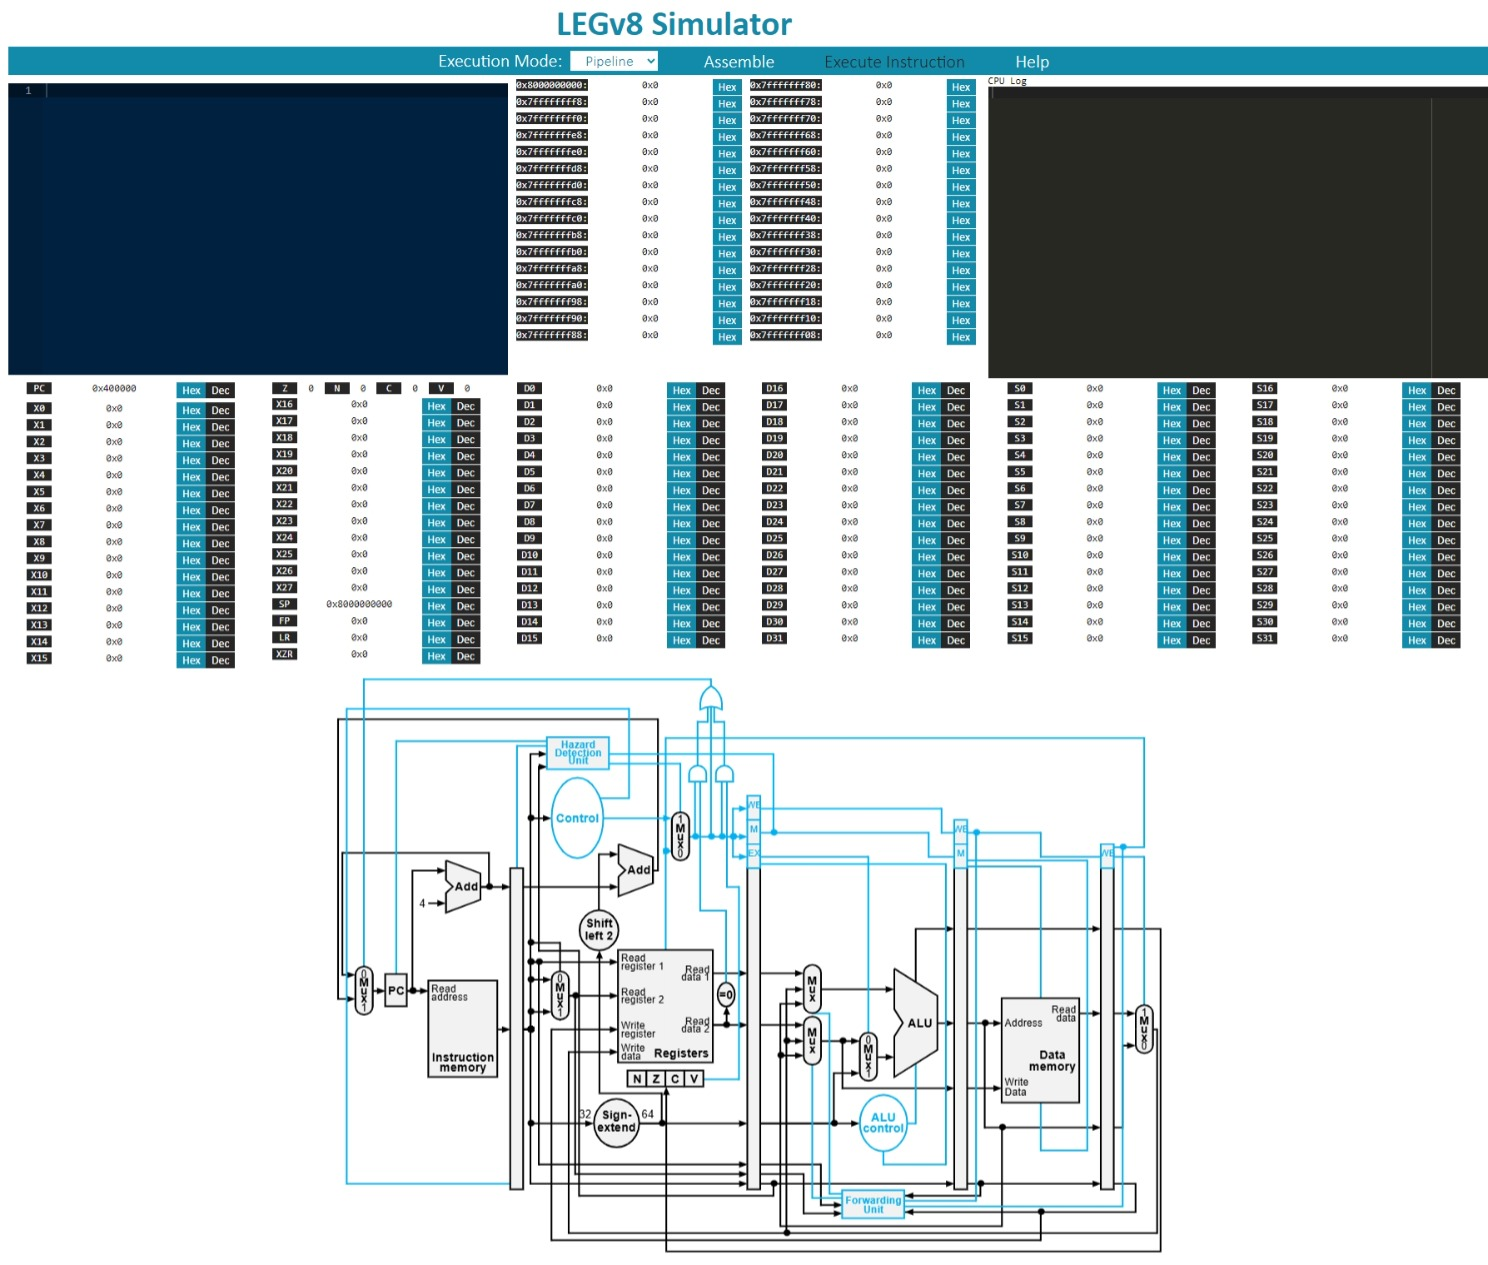
\includegraphics[width=1\textwidth]{img/new_pipeline.jpeg}
	}
	\caption{The updated pipeline UI}
\end{figure}